%% ------------------------------------------------------------------------- %%
\chapter{Usp Eventos}
\label{cap:uspeventos}
\section{Definição do Projeto}
\subsection{Motivação}
        \par A idéia de desenvolver um sistema utilizando Métodos Ágeis e conceitos de \emph{Lean Startup} surgiu em dezembro de 2015. O objetivo era desenvolver um sistema web ou aplicativo voltado para a comunidade USP com a intenção de facilitar de alguma forma o dia-a-dia dos usuários.
        \par Inicialmente existiam algumas propostas de projeto que foram então formalizadas em uma enquete realizada junto a comunidade USP.
\subsection{Enquete e definição do projeto}
        \par  No início as seguintes hipóteses de interesse de projeto foram disponibilizadas para votação:
                \begin{itemize}
                \item {USP avisa eventos e incidentes:} Um sistema para reportar desde eventos acontecendo no campus (palestras, festas, etc) até outros incidentes (buracos, perigos, etc).
                \item {USP doações e trocas: } Um sistema voltado para os membros da comunidade que desejam fazer doações ( sejam móveis, roupas usadas, etc) para outros e aqueles dispostos a receber. organizando filas de interesse,disponibilidade e urgência.
                \end{itemize}
        \par Com o intuito de entender melhor nosso público alvo, além de aberto a outras sugestões, foi necessario um sistema que suportasse não só uma votação fechada como também permitisse que os próprios usuários fossem capazes de adicionar outras propostas de forma dinâmica àquelas já existentes.
        \par O sistema POP (Painel de Opinião Pública) foi escolhido para efetuar a enquete pois permitia uma criação dinâmica de opções pelos usuários. Foi então criada uma instância independente do sistema adaptada chamada POP-TCC (figura \ref{fig:pop-tcc}) utilizando o Heroku que poderia ser acessada pelo endereço pop-tcc.herokuapp.com.
        \par Em 11/01 foi enviado o primeiro e-mail com a enquete do POP-TCC aberta para a lista de e-mails dos alunos do IME com as duas opções iniciais de projeto supracitadas. A divulgação da enquete concentrou-se principalmente via facebook nas seguintes comunidades:
\begin{figure}[htb]
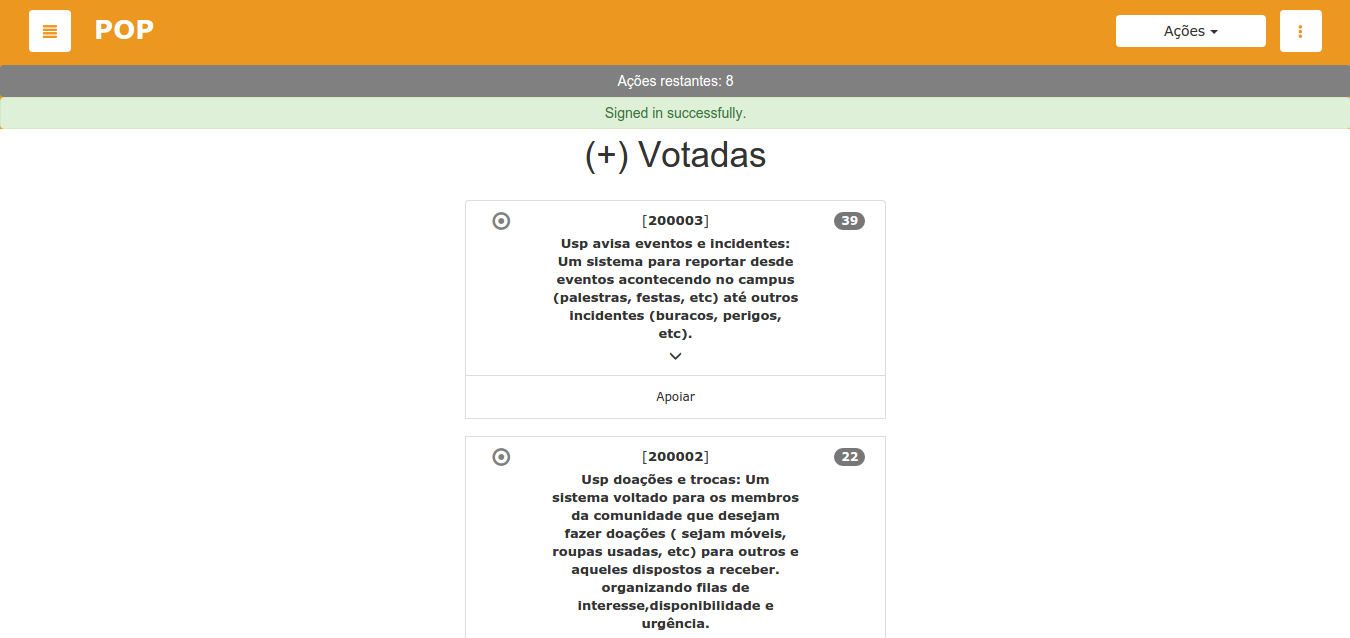
\includegraphics[width=15cm]{figuras/pop-tcc}
\caption{\label{fig:pop-tcc} Sistema POP-TCC com a enquete para votação.}
\end{figure}
\begin{table}[]
\centering
\caption{Comunidades do Facebook na qual foram feitas divulgações}
\label{my-label}
\begin{tabular}{ll}
{\color[HTML]{3531FF} \textbf{Comunidade}} & {\color[HTML]{3531FF} \textbf{Número de Membros}} \\
USP - Universidade de São Paulo            &                                                   \\
FAU USP                                    & 4000                                              \\
IME USP                                    & 3000                                              \\
Universidade de São Paulo                  & 5000                                              \\
Baladas USP                                & 15000
\end{tabular}
\end{table}
\par Ao longo de duas semanas outras opções de projeto surgiram. O resultado final \ref{fig:poll_chart} da enquete e a descrição das sugestões seguem abaixo:
\begin{itemize}
\item{ 1º Lugar (39 votos):} USP avisa eventos e incidentes: Um sistema para reportar desde eventos acontecendo no campus (palestras, festas, etc) até outros incidentes (buracos, perigos, etc).
\item {2º Lugar (21 votos):} USP doações e trocas: Um sistema voltado para os membros da comunidade que desejam fazer doações (sejam móveis, roupas usadas, etc) para outros e aqueles dispostos a receber; organizando filas de interesse, disponibilidade e urgência.
\item {3º Lugar (20 votos):} USP caronas: os motorizados colocam horário, bairro, quantidade de lugares disponíveis, ponte de embarque e desembarque. os interessados enviam um alerta para os motorizados confirmarem até preencherem as vagas.
\item {4º Lugar (18 votos):} Mapa de crimes na USP: um app onde roubos, furtos, assaltos, agressões, assédios, discriminações e outros crimes podem ser relatados, georreferenciados no campus.
\item {5º Lugar (14 votos):} Volta pedalusp - volta e desenvolvimento da ideia que já teve adesão, mas morreu por falta de manutenção. implementação de novos pontos de troca de bikes mais próximos das faculdades e outros pontos estratégicos.
\item {6º Lugar (13 votos): } USP extensão: uma plataforma de apoio mútuo para organização, contato, criação e divulgação de projetos de extensão dentro da universidade.
\item {7º Lugar (12 votos):} USP gigabyte: um ponto de encontro virtual pra reunir o pessoal e tomar uma rodada de suco com a galera. curtição, azaração e muita gente bonita neste, que é o ponto mais quente da internet!
\item {8ºLugar (8 votos):} Monitoria voluntária: pessoas divulgam horário e local no qual pessoas podem procurá-las para tirar dúvidas sobre certas disciplinas comuns a vários cursos.
\end{itemize}
\begin{figure}[htb]
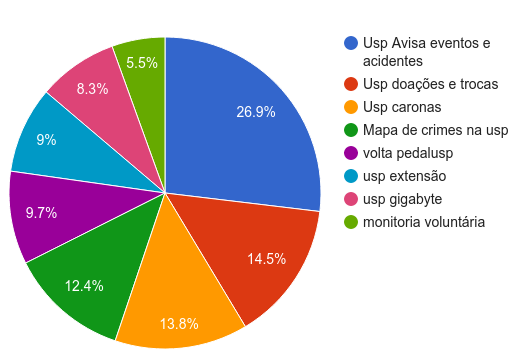
\includegraphics[width=10cm]{figuras/poll_chart}
\caption{\label{fig:poll_chart} Gráfico gerado pelo resultado da Enquete.}
\end{figure}
\par O projeto escolhido então foi o USP Avisa Eventos e Acidentes que seria renomeado apenas para USP Eventos.
\section{Definindo as características do Sistema}
\subsection{Pesquisa de Sistemas Semelhantes}
\par Definido o tema do projeto teve início uma pesquisa para levantar a existência de sistemas que tivessem uma proposta semelhante de divulgação de eventos e atividades.
\par Ao realizar essa pesquisa expandimos o escopo para que os sistemas não necessariamente fossem voltados para fins acadêmicos apenas tendo como objetivo principal obter uma base de conhecimento de quais funcionalidades um sistema de divulgação possui ou mesmo encontrar uma solução em código aberto que pudesse ser utilizada como base.
 \par Também foi enviado um e-mail em março para a lista de Representantes Discentes do próprio IME questionando sobre funcionalidades e sugestões.
\par Das compilações sobre a pesquisa e resposta obtidas por e-mail destacam-se 3 sites com proposta e conteúdos semelhantes:
\begin{itemize}
\item{Eventos USP (http://www.eventos.usp.br/):}
Canal de divulgação oficial da USP para eventos ocorrendo em suas dependências para todos os campus.\\
Pontos Fortes: Sendo o canal de comunicação oficial da universidade ele mostra-se com uma ótima fonte de conteúdo sobre eventos oficiais.\\
Pontos Fracos: É uma via de mão única na qual o usuário apenas se informa dos detalhes do evento mas não tem oportunidade de criar ou divulgar o seu próprio.
\item {Catraca-Livre (https://catracalivre.com.br/brasil/):} Principal Portal de atividades culturais e divulgação de eventos costuma ser bastante eclético. \\
Pontos Fortes: Apesar de não ter um conteúdo personalizável a página de Agenda possui uma grande variedade de opções de filtro.\\
Pontos Fracos: Como divulga eventos por toda a cidade sua navegação é bastante confusa levando o usuário a facilmente perder-se devido à grande quantidade de informações e poucas opções de personalização. Soma-se a isso o fato de que o site é uma forma de comunicação unilateral não permitindo que usuários divulguem e organizem seus próprios eventos.\\
\item {SP Cultura (http://spcultura.prefeitura.sp.gov.br/):} Portal oficial da prefeitura de São Paulo para divulgação de atividades por toda a cidade.\\
Pontos Fortes: Possui bastante opções de filtros além de permitir que um usuário interessado crie um evento e submeta-o para aprovação, bastante intuitivo e de fácil acesso. É baseado em uma solução de código aberto.\\
Pontos Fracos: Os eventos estão distribuídos por um mapa georreferenciado, dando mais ênfase à localização do evento do que sobre sua descrição obrigando o usuário a selecionar primeiro um evento em uma localização para então obter informações do mesmo.
\end{itemize}
\subsection{Plataforma Web x Móvel}
\par Para decidir em qual plataforma desenvolver nosso sistema foi levado em consideração fatores técnicos e do público-alvo.
\par De acordo com o gráfico \ref{fig:global_market_sharing} observa-se que as plataformas Android e IOS hoje em dia correspondem respectivamente à 86,2\% e 12,9\% do mercado mundial de sistemas operacionais móveis totalizando juntas 99,1\% do mercado o que significaria que ao desenvolver dois aplicativos nativos para ambas as plataformas corresponderia à ter a acesso à quase totalidade do mercado móvel. \footnote{Fonte: Statista \url{http://www.statista.com/statistics/254653/mobile-internet-user-penetration-in-brazil/} Acesso em: 22 out. 2016.}
\begin{figure}[htb]
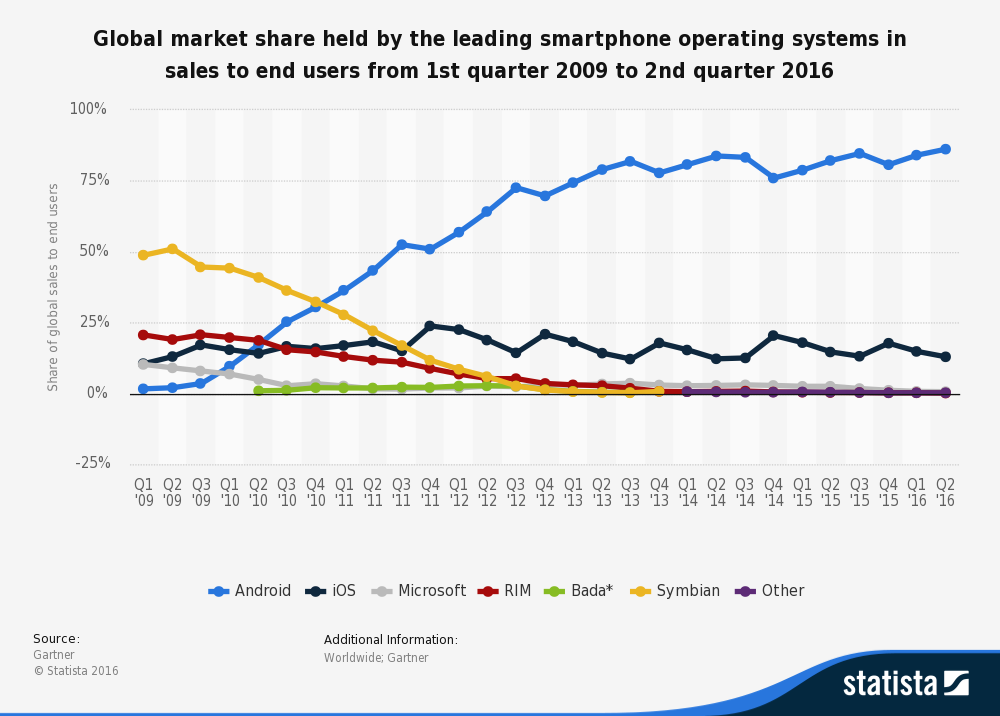
\includegraphics[height=10cm]{figuras/global_market_sharing}
\caption{\label{fig:global_market_sharing} Distribuição de mercado para Sistemas Móveis.}
\end{figure}
\par Foram feitas as seguintes considerações quanto ao desenvolvimento de uma aplicação nativa. \footnote{Fonte: Caelum \url{http://blog.caelum.com.br/aplicacoes-mobile-web-ou-nativa/} Acesso em: 22 out. 2016.}
\begin{itemize}
\item O desenvolvimento para Android é feito utilizando a linguagem Java a partir de APIs fornecidas pelo próprio Google enquanto um aplicativo para IOS utiliza Objective-c ou Swift por meio das APIs fornecidas pela Apple.
\par Devido a isso não há correspondência de código entre ambas plataformas tornando necessário o desenvolvimento de duas aplicações distintas caso queira-se atingir a totalidade do mercado.
\item Os aplicativos nativos seguem um padrão bastante rígido de UI/UX que divergem bastante entre si.
\par Os padrões de desenvolvimento para interfaces de um aplicativo Android diverge totalmente de um aplicativo IOS quanto a sua usabilidade e layout fazendo com que seja necessário pensar em duas interfaces distintas.
\item A maior vantagem de um aplicativo nativo é ter acesso aos recursos de \emph{hardware} do smartphone tais como câmera ou acelerômetro.
\par Como nossa aplicação não faria uso de nenhum recurso específico tais vantagens não seriam aproveitadas.
\item Os aplicativos nativos estão sujeitos às normas e aprovações de suas lojas virtuais, Play Store para o Android e Apple Store para o IOS, fazendo com que o tempo de publicação de uma atualização aumente devido a necessidade de aprovação da loja em questão.
\item Não seria possível utilizar a plataforma em Desktops restringindo o público-alvo.
\end{itemize}
\par A escolha de uma aplicação web deu-se principalmente pela facilidade de atualização de uma aplicação web por não necessitar da aprovação de um loja online ganhando em agilidade para realizar novos experimentos.
\par Apesar da escolha de um sistema web ao analisar o crescimento do acesso móvel no Brasil~\ref{fig:mobile_internet}, que vem aumentando a passos largos no país, houve a preocupação de desenvolver-se uma aplicação web híbrida com uma interface totalmente responsiva \footnote{ Uma interface responsiva de um site ou página é uma versão do layout adaptada para uso em telas menores comumente refere-se a visualização em smartphones} desde o princípio.
\begin{figure}[htb]
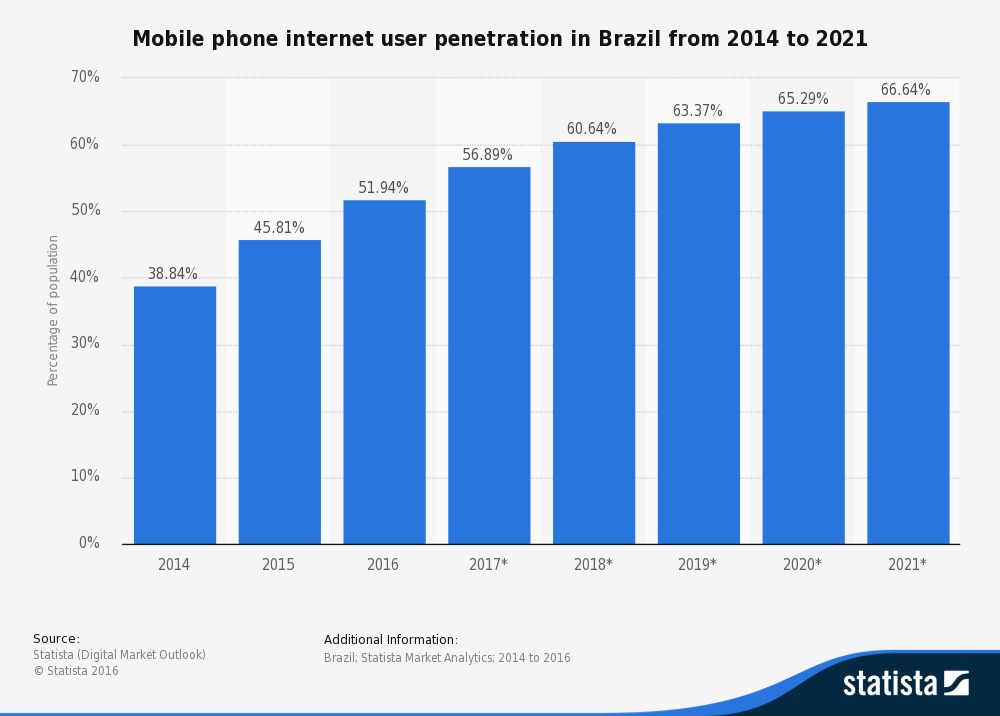
\includegraphics[height=10cm]{figuras/mobile_internet}
\caption{\label{fig:mobile_internet} Crescimento do Uso de internet móvel no Brasil.}
\end{figure}
\par Dessa forma apesar do acesso em um smartphone não ser tão intuitivo quanto em uma aplicação nativa ainda sim teria uma interface funcional garantindo que a navegação em uma plataforma móvel fosse feita sem dificuldades.
\subsection{Porque escolher Ruby on Rails }
\par O uso do \emph{Ruby on Rails} entre \emph{startups} tem crescido nos últimos anos isso devido a alguns fatores intrinsecamente ligados à própria estrutura do arcabouço Rails e também à necessidade que \emph{startups} e o próprio modelo de \emph{Lean Startup} exigem para iterações e alterações de códigos rápidas(\cite{lilia:16}).
\par Uma das principais filosofias do Ruby on Rails, o CoC \- Convenção sobre Configuração, permite que o desenvolvedor possa, a partir de um conjunto pré-definido de configurações padrões, agilizar o desenvolvimento do código ao tirar de sua responsabilidade fatores de configuração em detrimento de um padrão já estabelecido(\cite{morrice:15}).
\par Dessa forma desenvolvedor mais tempo para concentrar-se em decisões sobre o produto. Essa agilidade em codificar rapidamente resulta em interações mais rápidas contribuindo para uma maior agilidade dentro do ciclo de Construir-Medir-Aprender. Outro fator a favor do arcabouço Rails é o grande enfoque em testes automatizados(\cite{morrice:15}).
\par Para o desenvolvimento da plataforma USP Eventos foram utilizadas as gems Rspec e Capybara que permitem não só a realização de testes unitários como também testes de integração de modo muito rápido e direto garantindo assim a confiabilidade do projeto.
\par Soma-se a isso a quantidade enorme de ferramentas que auxiliam na integração contínua do código como por exemplo o Travis CI utilizado durante o desenvolvimento da plataforma.
\par O Travis CI era responsável para que a cada commit realizado fosse executada toda a bateria de testes automatizados enviando um e-mail contendo um relatório sobre o seu resultado, inclusive em caso de falha, garantindo dessa forma que todos tivessem sempre conhecimento das alterações sobre o código além de evitar problemas de conflitos de versões ou mesmo que uma atualização de projeto fosse colocada no ambiente de produção contendo alguma falha.
\par O fator comunidade é outra vantagem do RoR. Destacando-se pelo seu tamanho, interesse e acessibilidade em tirar dúvidas sempre contribuindo para promover o arcabouço a comunidade que orbita ao redor do Rails foi capaz de criar ferramentas prontas para uso com uma ótima documentação, tutoriais, cursos e guias garantindo assim que qualquer desenvolvedor interessado sempre tenha em mãos materiais e ferramentas de qualidade para iniciar o desenvolvimento do seu projeto.(\cite{lilia:16})
\par Acrescenta-se também à favor do arcabouço Rails sua escalabilidade. Rails é utilizado por empresas de grande porte tais como Groupon, Twitter, Basecamp, mostrando-se um arcabouço robusto capaz de lidar com grandes sistemas sem ter uma queda de desempenho.(\cite{lilia:16})
\par Para finalizar Rails é também um arcabouço seguro garantindo, mesmo em sua configuração padrão ou com o auxílio de alguns plugins, proteção contra SQL-Injections e XSS( \emph{Cross Site Scripting}).
\par Além disso os programadores que contribuem para o arcabouço devem seguir o \emph{Secure Life Cycle Development}, figura \ref{fig:security_dev_lifecycle}, proposto pela Microsoft, um modelo de desenvolvimento de software cujo principal objetivo é ajudar o a construir software mais seguros e confiáveis e reduzir custos \footnote{Fonte: Wikipedia \url{https://en.wikipedia.org/wiki/Microsoft_Security_Development_Lifecycle} Acesso em: 22 out. 2016.}.
\begin{figure}[htb]
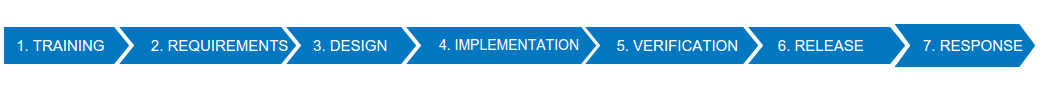
\includegraphics[width=15cm]{figuras/security_dev_lifecycle}
\caption{\label{fig:security_dev_lifecycle} Fases do Secure Life Cycle Development.}
\end{figure}
\section{Kanban}
\par Kanban é uma palavra japonesa e significa cartão visual para prover informação de regulamentação do fluxo de estoque e materiais. Possui três regras principais (KNIBERG, H., 2009): visualizar o fluxo de trabalho; limitar o trabalho em cada estágio do fluxo, e medir o tempo de avanço (tempo médio para se completar cada item). ( \cite{francisco:14})
\par No contexto de Métodos Ágeis e \emph{Lean Startup} foi utilizado uma abordagem utilizando o Kanban para definir as hipóteses de produtos, o escopo de desenvolvimento e as tarefas para serem executadas durante as etapas de desenvolvimento.
\par Tradicionalmente o kanban para desenvolvimento de Software possui 3 estágios ( \cite{francisco:14}):
\begin{itemize}
        \item TO DO: referente a requisitos que ainda estão aguardando para serem
desenvolvidos.
        \item DOING: referente a requisitos que estão sendo desenvolvidos.
        \item DONE. referente a requisitos que já finalizaram e foram devidamente
revisados e testados.
\end{itemize}
\par Cada item adicionado na fila de TO DO é chamada de tarefa. Uma hipótese à ser testada pode ser transformada em uma série de tarefas pequenas à serem completadas durante o período de desenvolvimento.
\par Caso seja necessário é possível quebrar uma tarefa grande em uma série de tarefas menores. Tomando como exemplo a tarefa de Implementar um filtro de eventos para a página principal. Ela foi quebrada em 3 tarefas menores para serem completadas: Implementar categorias de eventos, permitir adicionar categorias de eventos durante a criação de um novo evento e implementar filtro de eventos na página principal de eventos.
\par O tempo que uma tarefa demora desde sua entrada no quadro até a saída é denominado \emph{Lead Time}. Em um ambiente de \emph{startup} o intuito é sempre obter o menor Lead Time possível para tal é importante estar ciente da taxa de entrega que sua equipe de desenvolvimento é capaz de cumprir e sempre definir as tarefas de modo simples.
\par Para utililzação no projeto USP Eventos foi incluída uma coluna a mais denominada BACKLOG, comumente usada na metodologia Scrum \footnote{Fonte: Desenvolvimento Ágil \url{fonte http://www.desenvolvimentoagil.com.br/scrum/sprint_backlog} Acesso em: 22 out. 2016.}, na qual foram colocadas ideias que poderiam ou não serem transformadas em tarefas de desenvolvimento ou hipóteses para serem executadas em uma iteração do ciclo de Construir-Medir-Aprender.
\par Em cada iteração do ciclo foi especificado quais hipóteses seriam testadas e a partir delas criado tarefas para serem implementadas.
\par Caso um bug fosse detectado uma tarefa era criada na fila de TO DO para resolvê-la.
\par A ferramenta Trello, figura \ref{fig:kanban}, foi utilizada para simular um quadro Kanban digital, com ela foi possível guiar todo o desenvolvimento do sistema.
\begin{figure}[htb]
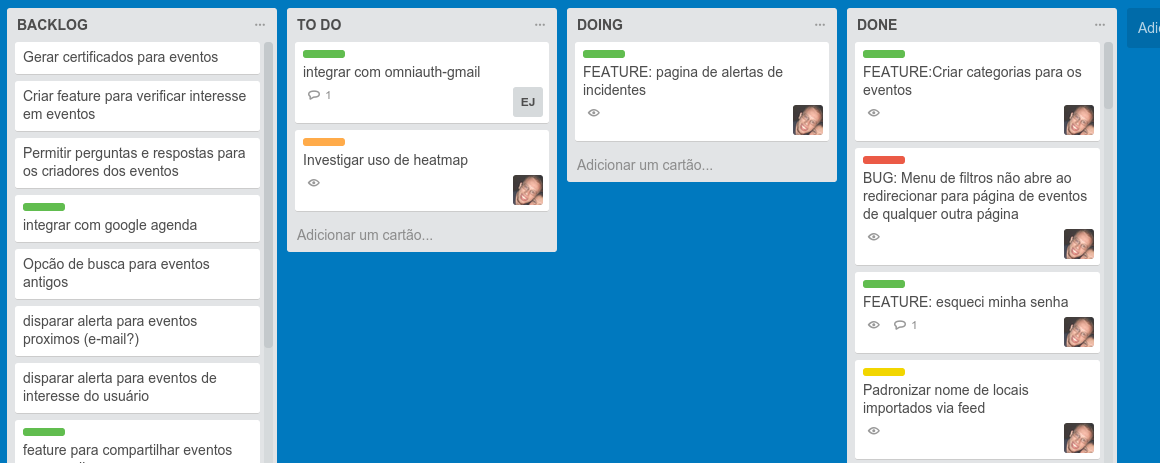
\includegraphics[width=15cm]{figuras/kanban}
\caption{\label{fig:kanban} Sistema Trello contendo as 4 colunas utilizadas no USP Eventos.}
\end{figure}
        Com o intuito de tornar melhor a visualização no Trello foram criados alguns Rótulos de cores distintas para cada tarefa:
        \begin{itemize}
        \item BUG (vermelho): Defeito não previsto durante o desenvolvimento.
        \item FEATURE (verde): Nova funcionalidade para ser implementada.
        \item REFACTOR(lilás):  Melhoria de código sem refletir uma mudança externa.
        \item MELHORIAS(laranja): Investigar ou implementar o uso de ferramentas externas ao sistema, tal qual a integração com o Google Analytics por exemplo.
        \item QUICK WIN(amarelo): Melhoria feita rapidamente e não prevista durante a definição de tarefas.
        \end{itemize}
\section{Primeira Iteração}
\subsection{Construção}
< em desenvolvimento>
         \par O primeiro MVP do USP Eventos tinha como objetivo testar as seguintes hipóteses:
         \begin{itemize}
         \item Medir o interesse do público em participar de um evento.
         \item Criar uma interface intuitiva e rápida para mostrar informações de eventos para o usuário.
         \end{itemize}
        \par A Página inicial (figura \ref{fig:landing_pagev1}) do site possuía acesso para a página de cadastro e login além de um formulário para envio de sugestões.
        \begin{figure}[htb]
		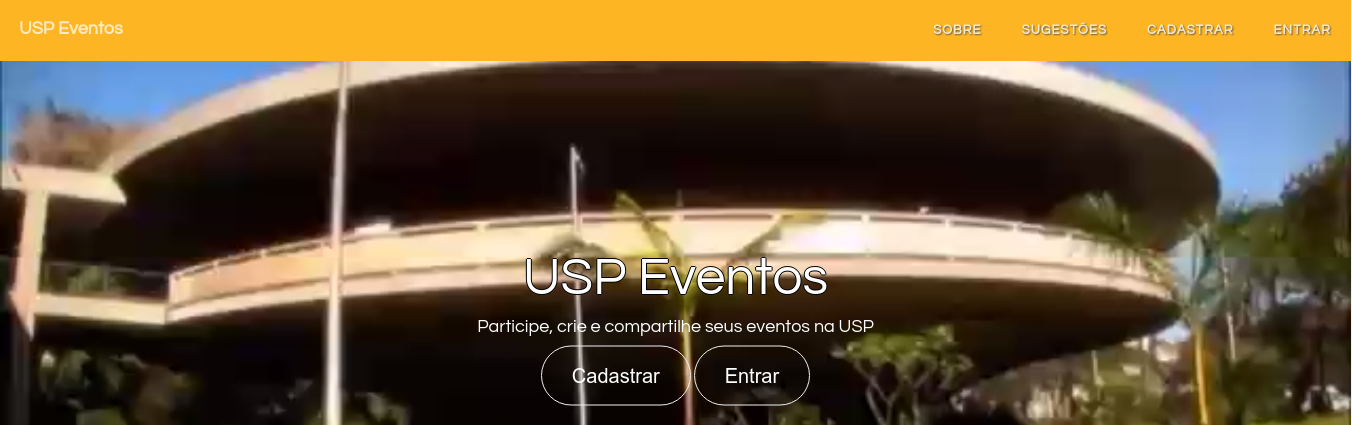
\includegraphics[width=15cm]{figuras/landing_pagev1}
		\caption{\label{fig:landing_pagev1} Tela inicial na primeira iteração }
		\end{figure}
        \par O cadastro de usuário (figura \ref{fig:sign_upv1}) pedia apenas nome, e-mail e senha inicialmente porém ainda na primeira iteração foi implementada a opção de login com facebook.
        \begin{figure}[htb]
		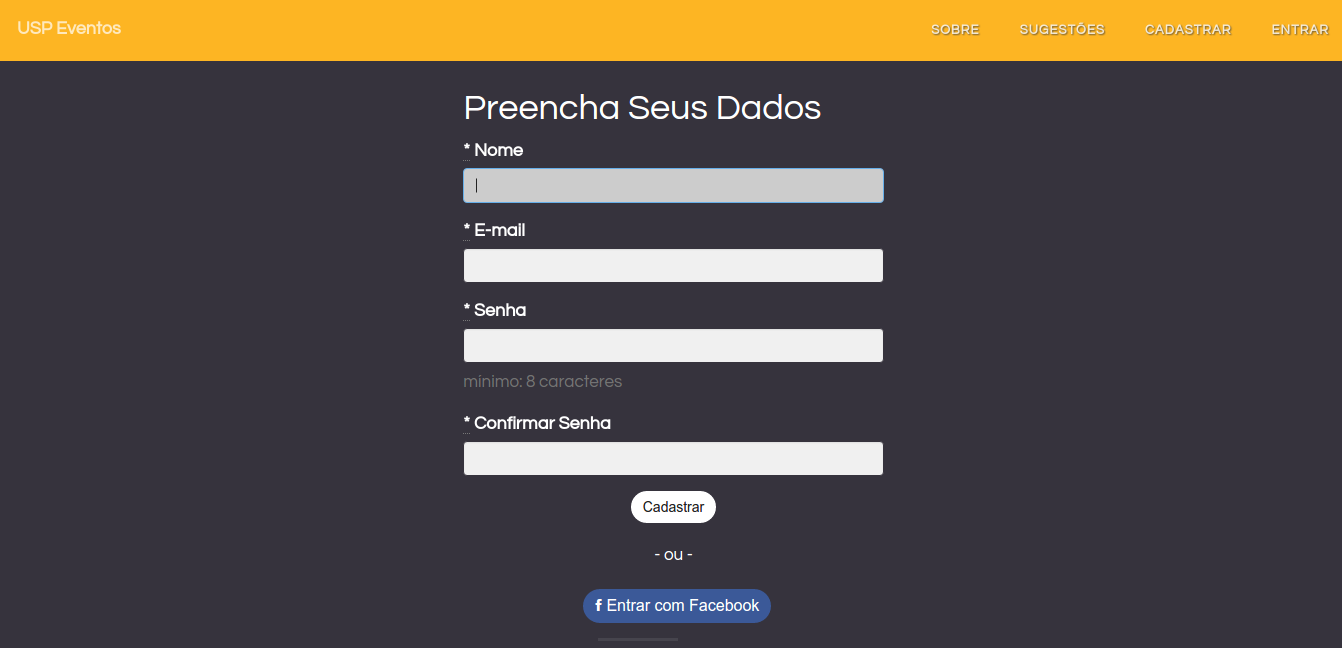
\includegraphics[width=15cm]{figuras/sign_upv1}
		\caption{\label{fig:sign_upv1} Tela de Cadastro na primeira iteração}
		\end{figure}
		\par A página de eventos (figura \ref{fig:events_pagev1}) só poderia ser acessada por um usuário logado tornando essa página e qualquer página de evento específica inacessível para um visitante sem login. Além disso a página de eventos apenas mostrava-os sem oferecer qualquer opção inicial de filtro.
        \begin{figure}[htb]
		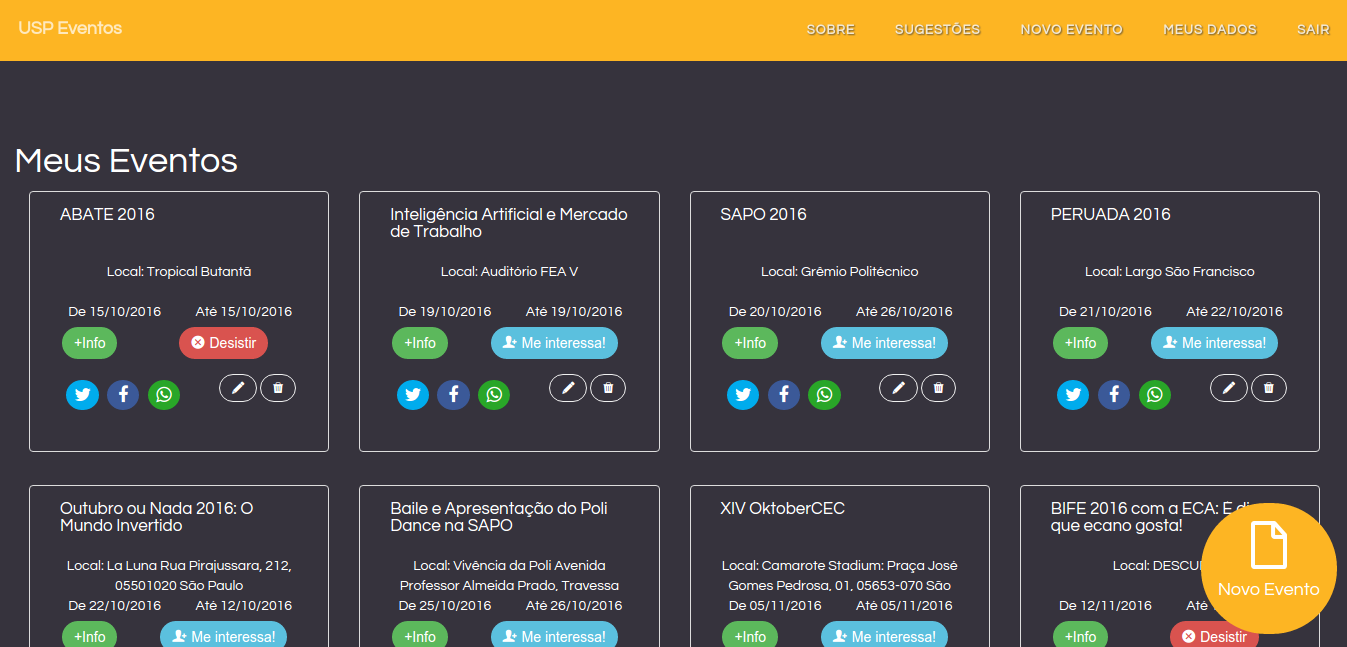
\includegraphics[width=15cm]{figuras/events_pagev1}
		\caption{\label{fig:events_pagev1} Página de Eventos}
		\end{figure}
\par Todas as páginas foram pensadas também para o acesso via mobile possuindo versões responsivas ( figura \ref{fig:events_pagev1_responsive}).
        \begin{figure}[htb]
		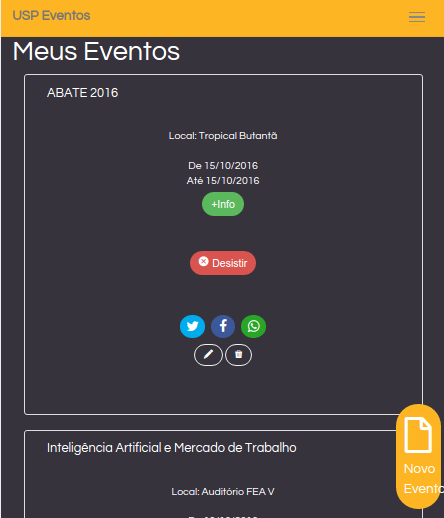
\includegraphics[width=5cm]{figuras/events_pagev1_responsive}
		\caption{\label{fig:events_pagev1_responsive} Página de Eventos versão responsiva}
		\end{figure}
\par Visando evitar que os usuários se depararem com uma página de eventos vazia foi feita uma \emph{Rake Task} \footnote{Rake é um programa implementado em \emph{Ruby} que permite ao usuário implementar \emph{tasks} que são executadas ao serem chamadas} para consumir o xml gerado pelo feed RSS que o site www.eventos.usp.br. Dessa forma seria possível adicionar de forma mais ágil alguns eventos dentro da plataforma.
\par Cada thumbnail de eventos presente na página principal de listagem de eventos incluía o nome do evento, localização, data de início e fim além de um botão de ``Participar'' para que os usuários que estivessem logados e também botões para compartilhamento nas principais redes sociais.
\par Houve também a preocupação de espalhar formulários de Sugestões em diversos pontos do site com o intuito de facilitar a coleta de informações do usuário.
\subsection{Divulgação}
\par A primeira versão do sistema ficou disponível a partir do dia 5 de maio e sua divulgação foi feita pelo facebook por grupos e comunidades associadas a institutos da USP tais como FFLCH, FAU, IME, ECA, assim como foram enviadas mensagens para as respectivas empresas Júnior e Atléticas.
\par Também foi divulgado a primeira versão na lista de alunos e representantes discentes do próprio Instituto de Matemática e Estatística.
\subsection{Métricas}
\par Para medir o fluxo de usuários dentro do site foi utilizado Google Analytics em conjunto com o Google Tag Manager.
\par Como métrica chave escolhemos medir a quantidade de usuários que se interessavam por um evento.
\par Foi criada então uma tag (figura \ref{fig:tags}) para rastrear os cliques no botão ``Participar'' presente dentro do thumbnail de um evento na página principal e também na página de detalhes do evento. Dessa forma seria possível mapear o interesse do usuário em um determinado evento.
\begin{figure}[htb]
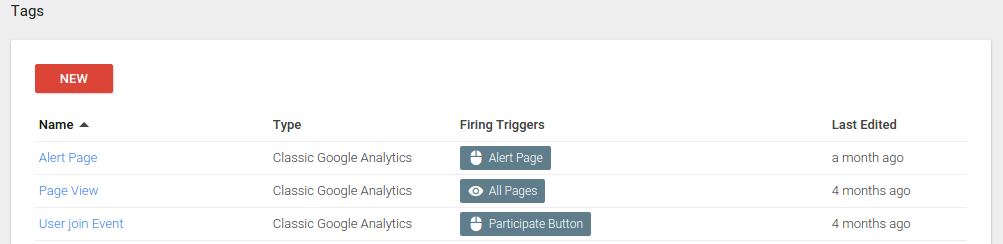
\includegraphics[width=15cm]{figuras/tags}
\caption{\label{fig:tags} Visualização das Tags pelo Google Tag Manager.}
\end{figure}
\par Em pararelo foi possível obter também por meio do Google Analytics as seguintes informações (figura \ref{fig:analytics_1interacao_dados}):
\begin{itemize}
\item Visualizações de Páginas: ``Exibições de página'' refere-se ao número total de páginas visualizadas. Exibições repetidas de uma única página são consideradas.
\item Páginas / Sessão: Número total de sessões \footnote{Uma sessão é o período que um usuário fica ativamente engajado com seu website, aplicativo, etc. Todos os dados de uso (exibições de tela, eventos, comércio eletrônico etc.) são associados a uma sessão.} no período.
\item Duração Média da Sessão: Auto-explicativo.
\item Usuários: Os usuários que realizaram pelo menos uma sessão no período selecionado. Inclui usuários novos e recorrentes.
\item Taxa de Rejeição: A taxa de rejeição é a porcentagem de visitas a uma única página (ou seja, visitas nas quais a pessoa sai de seu site na mesma da página de entrada, sem interagir com a página).
\item Porcentagem de Novas Sessões: Uma estimativa da porcentagem de primeiras visitas.

\end{itemize}

\begin{figure}[htb]
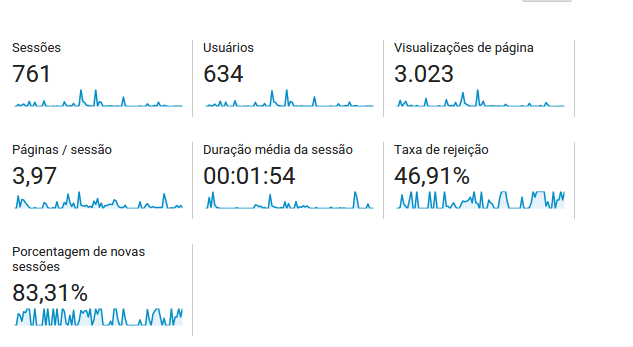
\includegraphics[width=15cm]{figuras/analytics_1interacao_dados}
\caption{\label{fig:analytics_1interacao_dados} Dados obtidos pelo G.A de 01/05 até 31/07}
\end{figure}

\par É possível observar uma grande taxa de rejeição inicial ao site no período associado principalmente na página inicial com cerca de 761 sessões e 423 desistências (figura \ref{fig:analytics_1ainteracao_fluxo}).
\par Durante o período observado foram registrados apenas 184 cliques em 56 sessões únicas no botão ``Participar''.
\begin{figure}[htb]
\centering
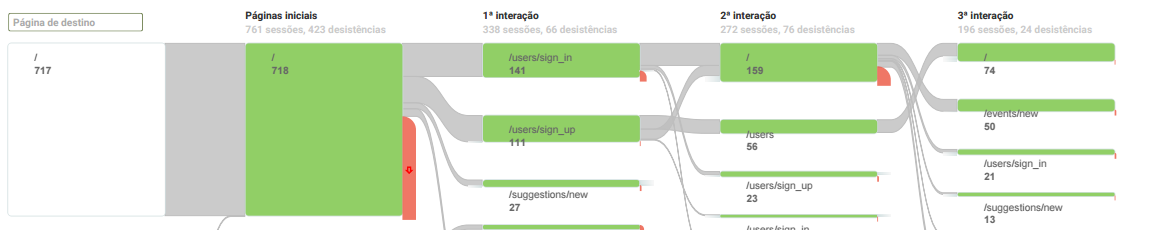
\includegraphics[width=15cm]{figuras/analytics_1ainteracao_fluxo}
\caption{\label{fig:analytics_1ainteracao_fluxo} Fluxo de Comportamento de 01/05 até 31/07.}
\end{figure}
\par A partir do gráfico de uso por tipo de Sistema Operacional (figura \ref{fig:analytics_1interacao_so})foi possível observar que a grande maioria dos usuários acessa o site por meio \emph{notebooks} ou computadores pessoais.
\begin{figure}[htb]
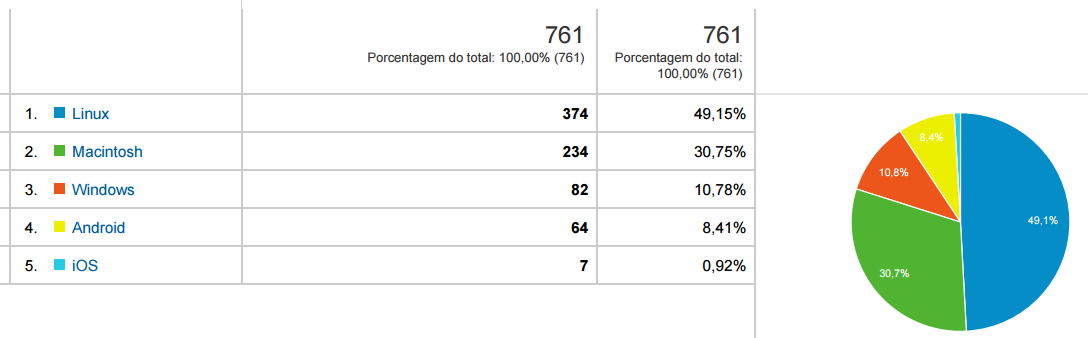
\includegraphics[width=15cm]{figuras/analytics_1interacao_so}
\caption{\label{fig:analytics_1interacao_so} Porcentagem de uso por S.O de 01/05 até 31/07.}
\end{figure}
\subsection{Aprendizado}
\par O maior número de acesso de usuários deu-se sempre em seguida aos posts realizados pelo facebook, alcançando picos de acesso mostrando a importância da divulgação pela plataforma.
\par Foi observado que os usuários acessavam o site porém não realizavam cadastro deixando-o logo em seguida resultando em um número elevado de desistências na página inicial.
\par Dentre os retornos recebidos pelo formulário do site, e-mails e de forma direta foram compiladas algumas críticas e sugestões:
\begin{itemize}
\item Página de eventos e visualização dos mesmos deveriam ser abertas para usuários mesmo sem login.
\item Ausência de um filtro de usuários tornou a página de eventos confusa para navegação.
\item Botão lateral de adicionar evento estava muito grande e atrapalhando a navegação.
\item Falta de cores na página principal tornou cansativa a navegação.
\item Clicar no nome do do evento no thumbnail para acessar a página do mesmo.
\item Ausência de opção de ``esqueci minha senha''.
\item Clicar no botão ``Participar'' não tinha uma utilidade prática. O evento era salvo porém isso gerava nenhum reflexo no sistema não existindo uma funcionalidade que justificasse sua existência e não havendo razão para que os usuários clicassem no botão.
\par Alguns comentários selecionados:

\par Por Veronica: ``Seria muito legal poder filtrar os eventos por tags referentes ao local / tipo / assuntos que serão abordados!''

\par Por Lucas: ``Olá! Eu gostaria de ver os eventos por categoria/área de conhecimento (Artes, História, Economia, Engenharia, etc).''

\par Por Carolina: ``Por que devemos nos cadastrar simplesmente para acessar o site? E se a pessoa ``simplesmente quer se informar sobre o que está acontecendo''? A minha sugestão é que somente quem quer enviar eventos para o site deveria se ter que se cadastrar. Obrigada e boa sorte no TCC.''

\par Por Karina: ``. [Login] Aos usuários que não possuem conta, mas tentam logar, seria ideal que o sistema mostra-se quando o usuário colocou dados incorretos e quando o usuário não possui conta.
\\
. [Página de eventos] Seria melhor que a célula do evento permitisse o click para adentrar detalhes sobre o mesmo
\\
. [Página de eventos] Inserir algumas ferramentas de filtro: datas (inicio/final ou datas pontuais); tags (algumas tags pré-cadastradas); campus;
\\
. [Página de eventos] Espaço para uma imagem nas células de divulgação do evento daria mais cor e chamaria mais a atenção dos usuários
\\
. Página de eventos] Seria legal colocar um aviso de inscrições limitadas para eventos que têm tal restrição''

\end{itemize}
\section{Segunda Iteração}
\subsection{Construção}
\par Levando em consideração o aprendizado da primeira iteração foi feita uma mudança no fluxo do site para permitir o acesso para a página de eventos sem a necessidade de realizar um cadastro antes ou exigir um \emph{login} do usuário.
\par As hipóteses a serem testadas foram:
\begin{itemize}
\item Verificar se as alterações visuais foram bem aceitas
\item Testar a hipótese da necessidade de Filtro para Eventos
\end{itemize}
\par Foi criado um filtro para a página de eventos baseado na utilização de tags dessa forma ao criar um novo evento (figura \ref{fig:event_newv2} )o usuário agora pode escolher 3 dentre 12 tags pré-definidas que servirão como filtro nas página principal.
        \begin{figure}[htb]
        \centering
		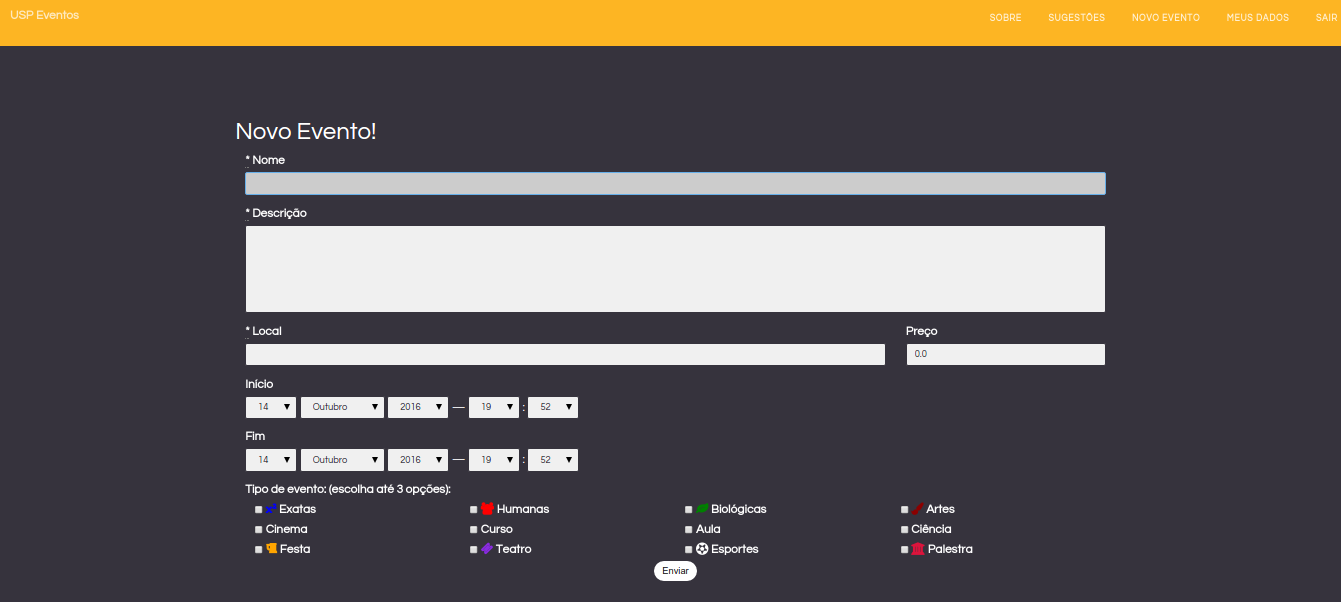
\includegraphics[width=15cm]{figuras/event_newv2}
		\caption{\label{fig:event_newv2} Página de Cadastro de Novos eventos com filtros}
		\end{figure}

\par Visando tornar a navegação dentro da página de eventos mais fluída e menos cansativa foram realizadas algumas modificações visuais na exibição dos eventos (figura \ref{fig:events_pagev2})
\begin{itemize}
\item Remodelagem do thumbnail de Eventos
\item Diminuição do botão de adicionar novos eventos para não atrapalhar a navegação
\item Adição de um menu lateral com opções de Filtros para os eventos
\item Nova listagem personalizada de Eventos segundo os interesses do usuário
\end{itemize}
        \begin{figure}[htb]
        \centering
		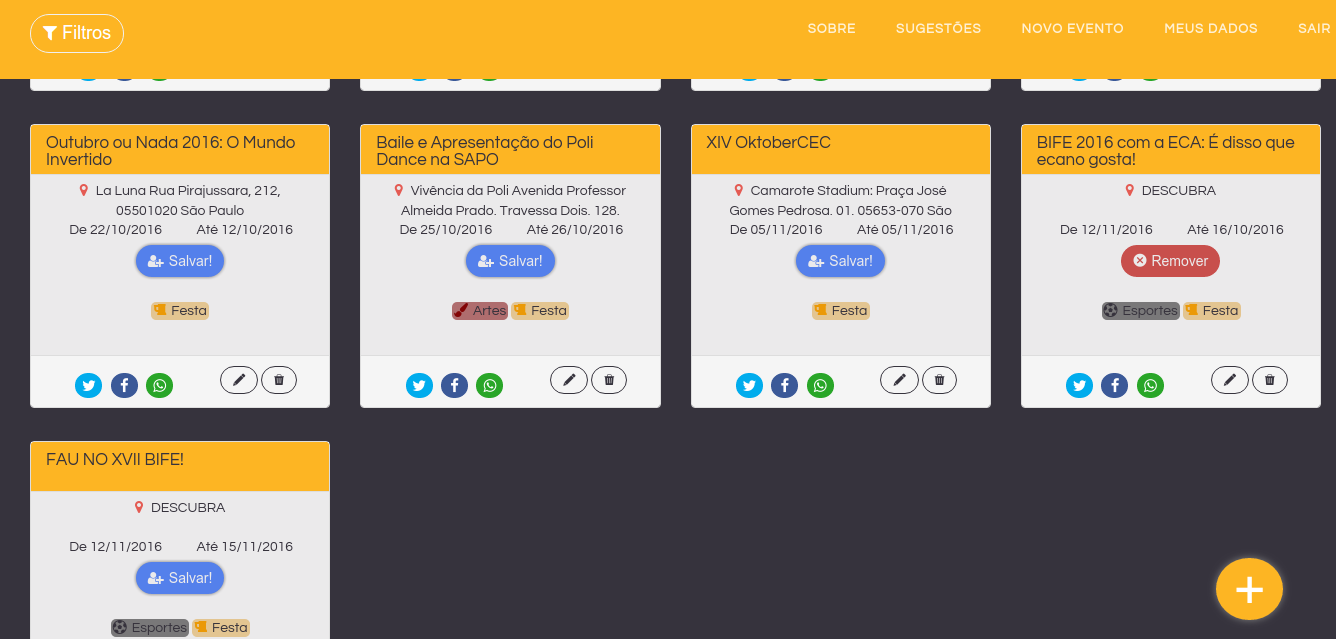
\includegraphics[width=15cm]{figuras/events_pagev2}
		\caption{\label{fig:events_pagev2} Página de Eventos com as alterações para a segunda iteração}
		\end{figure}

\par Os filtros (figura \ref{fig:events_pagev2_filters}) estão em um menu lateral que é acionado por um botão na parte superior esquerda. Também é possível selecionar cada \emph{tag} individualmente ao clicar sobre a respectiva nos \emph{thumbnails} de eventos.
        \begin{figure}[htb]
		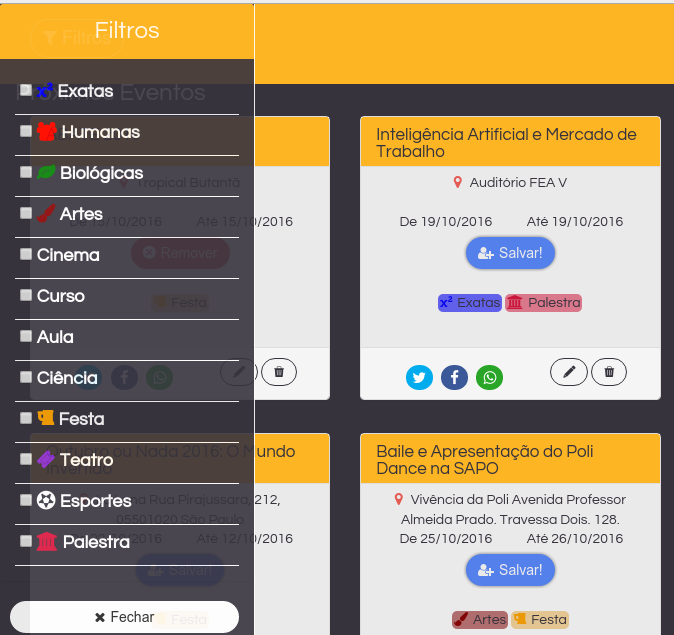
\includegraphics[width=15cm]{figuras/events_pagev2_filters}
		\caption{\label{fig:events_pagev2_filters} Filtros na página de Eventos}
		\end{figure}
As mudanças realizadas (figura \ref{fig:thumbs_comparison_v1_v2}) no thumbnail de eventos:
\begin{itemize}
\item Removido botão de +Info, agora para acessar mais informações basta clicar sobre o nome do evento
\item Adicionado Cabeçalho para separar e dar maior ênfase para o título e uma cor de fundo para aumentar o contraste com o plano de fundo a fim de facilitar a leitura
\item Adição de tags com as classificações dos eventos facilitando a escolha do mesmo.
\item Mudança do nome do botão de ``Participar'' para ``Salvar''
\end{itemize}
        \begin{figure}[htb]
        \centering
		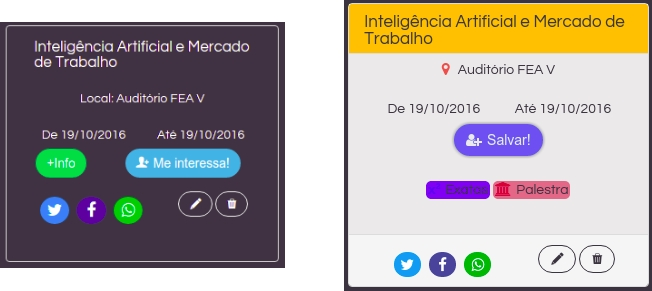
\includegraphics[width=15cm]{figuras/thumbs_comparison_v1_v2}
		\caption{\label{fig:thumbs_comparison_v1_v2} Esquerda: versão antiga. Direita: Versão atualizada}
		\end{figure}

\par Em conjunto com a criação das tags para eventos foi criado um mecanismo de preferências para o usuário, agora na página de cadastro ou edição de usuário é possível selecionar as tags com as quais o usuário tenha maior afinidade com o intuito de exibir uma listagem personalizada de eventos segundo esses critérios.
\par Aproveitando o sucesso do lançamento do aplicativo Pokémon GO \footnote{Fonte: Pokemon GO \url{ https://en.wikipedia.org/wiki/Pokemon_Go } Acesso em: 12 out. 2016.} que gerou uma enorme quantidade de acessos e movimentação pelo Campus foi criado uma página de Alertas \ref{fig:alert_page} no Campus visando atingir o público que estava utilizando o aplicativo para divulgar a localização de Pokémons.
\begin{figure}[htb]
\centering
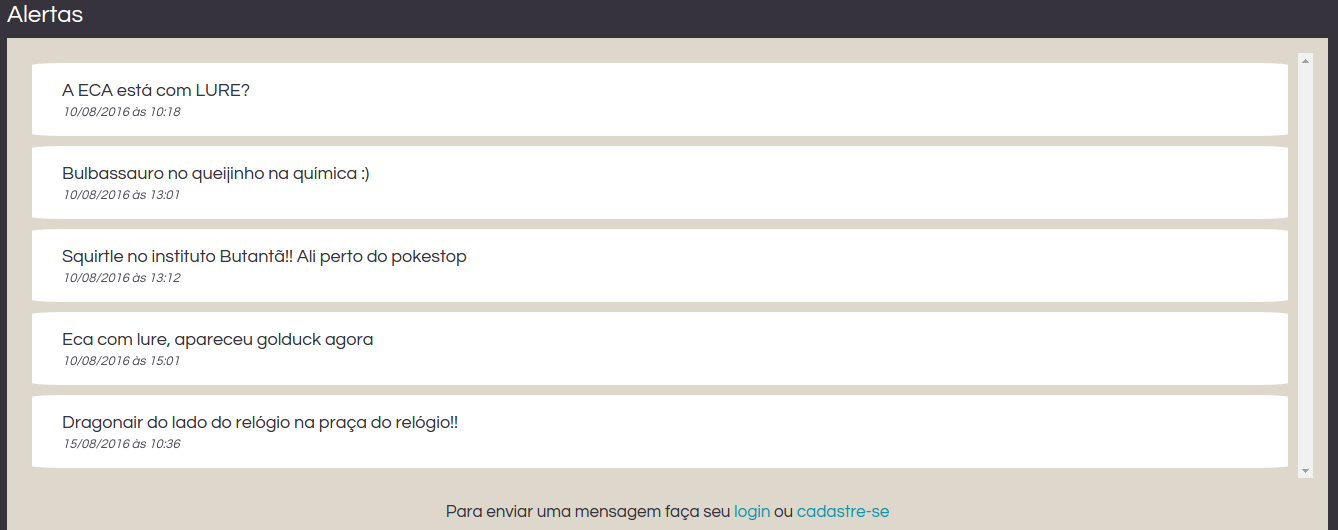
\includegraphics[width=15cm]{figuras/alert_page}
\caption{\label{fig:alert_page} Página de Alertas}
\end{figure}
\par A implementação de um testes para a página de Alertas tão rapidamente só foi possível devido a grande flexibilidade que o modelo de Construir-Medir-Aprender oferece pois somente assim foi possível rapidamente integrar uma nova funcionalidade não prevista dentro do escopo do projeto e medir sua eficácia.
\par Além disso com o auxílio de testes automatizados, ferramentas para integração contínua e a agilidade do desenvolvimento em Rails foi possível desenvolver e colocar as alterações no ambiente de produção sem comprometer a integridade do sistema como um todo.

\par Por fim foi adicionada uma página ``Sobre'' com informações sobre os responsáveis pelo site assim como seus objetivos.
\subsection{Divulgação}
\par Além da divulgação pelo facebook foram espalhados cartazes em pontos estratégicos pela USP tais como Pontos de Ônibus com grande movimentação, murais próximos aos Bandejões e também no interior de alguns institutos.

<fotos cartazes no pontos de onibus>

\subsection{Métricas}

\par Foi mantido o rastreamento pelo google Analytics do botão ``Participar'' porém seu nome foi alterado para ``Salvar'' com o intuito refletir melhor sua utilidade: Salvar um evento como interessante para exibi-lo na seção de ``Meus Eventos'' da listagem de eventos do usuário.

\par A nossa métrica chave continuou sendo avaliar o interesse dos usuários em determinado Evento por meio do clique no botão ``Salvar''.

\par A partir dos resultados obtidos pelo Googgle Analytics ((figura \ref{fig:analytics_2ainteracao_dados}) foi observado uma diminuição no número de sessões, entretanto também houve uma diminuição significativa na taxa de rejeição do site caindo de 46,91\% para 33,16\%.
\par O tempo médio por sessão também aumentou passando de 1:54 minutos para 3:37 minutos. Mostrando um aumento na retenção de usuários acessando a plataforma.
\begin{figure}[htb]
\centering
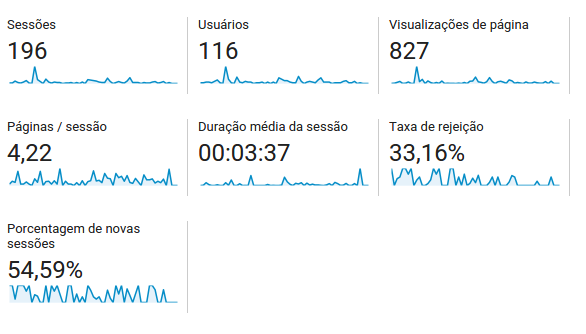
\includegraphics[width=15cm]{figuras/analytics_2ainteracao_dados}
\caption{\label{fig:analytics_2ainteracao_dados} Dados obtidos pelo G.A de 01/08 até 30/09}
\end{figure}

\par Com o lançamento da seção de Alertas foi feita uma divulgação via Facebook incentivando os usuários a utilizarem a plataforma com o intuito de divulgar a localização de Pokemons.
\par Foi colocado também uma \emph{tag} para rastrear o número de clicks no botão ``Alertas'' com a intenção de medir o interesse na funcionalidade, dessa forma foram observados 305 cliques no botão ``Alertas'' no período.

\par Analisando o gráfico de divisão por tipo de Sistema Operacional ((figura \ref{fig:analytics_2ainteracao_so}) percebemos que o acesso pelo sistema Android proporcionalmente mais que dobrou em relação ao período anterior, passando de 8,4\% para 19,36\%.

\begin{figure}[htb]
\centering
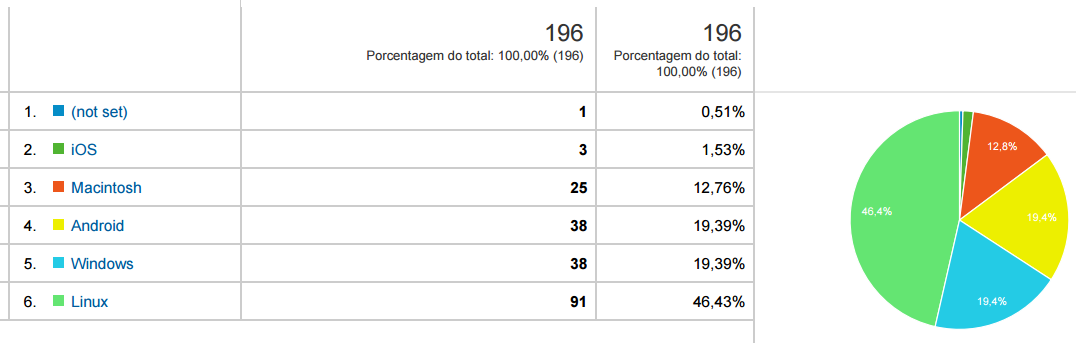
\includegraphics[width=15cm]{figuras/analytics_2ainteracao_so}
\caption{\label{fig:analytics_1interacao_so} Porcentagem de uso por S.O de 01/08 até 30/09.}
\end{figure}

\subsection{Aprendizado}

\par Com a abertura da página principal de Eventos, sem a obrigatoriedade de um cadastro, mais acessos foram registrados, porém quase não houveram novos cadastros dificultando assim que um usuário salvasse algum evento para sua lista.

\par Com a divulgação por cartazes foi possível constatar um aumento na utilização em dispositivos móveis principal forma de acesso em lugares públicos e incentivada devido ao QR Code presente nos cartazes.

\par Apesar do pico de acessos com o lançamento da página de Alertas a funcionalidade foi abandonada pelos usuários, gerando poucos acessos mostrando que talvez não fosse interessante investir em seu desenvolvimento.

\par Mesmo com a criação e filtros e melhorias visuais a página principal ainda carecia de apelo para navegação.
\par Alguns comentários recebidos de forma oral afirmaram que a página de eventos estava pouco atrativa visualmente sendo necessário que ela tivesse mais elementos que prendessem a atenção do usuário.

\par Novamente recebemos comentários pelo próprio formulário do site sobre adicionar a opção de incluir uma foto ao evento, segue: ``Sinto falta de anexo para cartazes. poder enviar uma foto ou cartaz escaneado do evento.'' - Ferdinand Machado

\section{Terceira Iteração}
\subsection{Construção}
	\par As maiores críticas recebidas durante a última iteração foram em relação a experiência proporcionada pelo site que não estava atrativa o suficiente. A partir desse \emph{feedback} foi decidido testar a seguinte a hipótese:
	\par - Melhorar a UX do site para aumentar a aceitação dos usuários.
	\par Em seu artigo publicado na \emph{Agile Conference} Beverly May (\cite{beverly:2012}), especialista em UX, discute alguns dos erros que cometeu o aplicar o método de \emph{Lean Startup}. Dentre eles um dos principais foi negligenciar a UX inicialmente. Como recomendação ele aconselha investir numa boa experiência de usuário sempre construindo protótipos e \emph{wireframes} \footnote{ Um wireframe web é uma ilustração semelhante do layout de elementos fundamentais na interface. , fonte \url{https://pt.wikipedia.org/wiki/Website_wireframe} Acesso em: 12 out. 2016.} antes de implementar para testar as modificações visuais.
	 \par Berverly também enaltece a importância de realizar testes constantes e sempre levar em consideração os \emph{feedbacks} dos usuários, positivos e negativos, um conceito também presente no ciclo de Construir-Medir-Aprender e base para o \emph{Customer Development}. No caso do USP Eventos foi feito um \emph{wireframe} ((figura \ref{fig:wireframe}) da página principal de Eventos com as modificações realizadas na iteração atual.
\begin{figure}[htb]
\centering
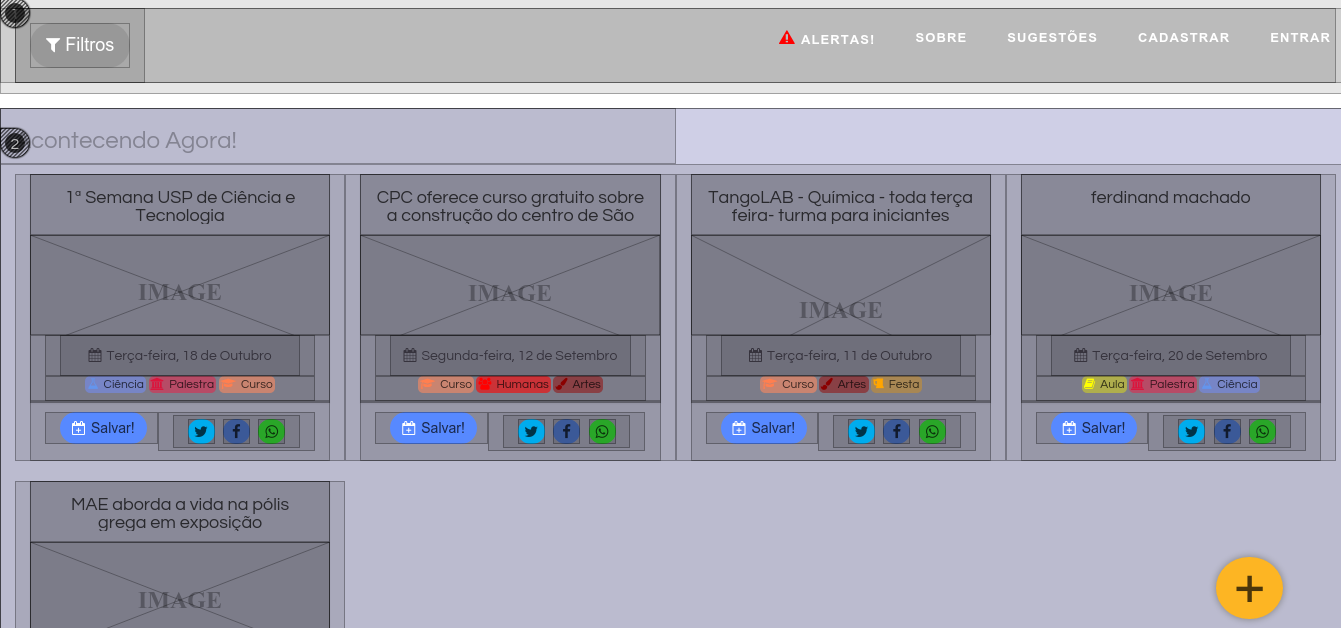
\includegraphics[width=15cm]{figuras/wireframe}
\caption{\label{fig:wireframe} Wireframe da versão modificada durante a Terceira Iteração}
\end{figure}
\par Para contornar a falta de conhecimento na área de \emph{User Experience} foram feitas pesquisas utilizando a bibliografia disponível e também entrevistas com profissionais da área. Isso melhorou a exibição de informação dentro do site, centralizando as principais modificações de UX na página de Eventos seguindo alguns preceitos apresentados por Steve Krug em seu livro ``Don't make me think'' (\cite{krug:00}), dentre eles:
	\begin{itemize}
	\item Eliminar distrações desnecessárias: Eliminar espaços em brancos e textos que possam distrair, poluir visualmente a página ou criar algum tipo de ruído na informação exibida.
	\item Criar hierarquias visuais claras: Dar mais destaque para as informações importantes e aproximar visualmente elementos que possuam ligações lógicas entre eles como nome do evento e sua data.
	\item Tirar vantagens de convenções: Utilizar layouts já consolidados de sites semelhantes para criar uma identificação na forma de navegar do usuário.
\end{itemize}
	\par Além disso para eliminar o excesso de texto presente na exibição de eventos e incluir mais informações visuais foi implementada uma opção de realizar \emph{upload} de uma imagem para o evento que seria exibida tanto na página principal de eventos como na página de informações gerais.
\par As modificações principais feitas foram (figura \ref{fig:events_page_3aiteracao}):
\begin{itemize}
\item Diminuir os espaços em branco dentro do thumbnail de Eventos deixando-o mais compacto.
\item Modificação nas cores e tamanho para dar destaque ao título, criando uma hierarquia visual a partir dele com as suas informações contidas no interior do \emph{thumbnail}.
\item Eliminação da exibição do local e data de término do evento para diminuir a poluição visual.
\item Presença de uma imagem identificadora no evento ao centro do thumbnail e em sua página de exibição.
\item O botão de “Salvar” deixou de estar localizado ao centro para ficar associado com os outros botões de compartilhamento na parte inferior do \emph{thumbnail}.
\end{itemize}
\begin{figure}[htb]
\centering
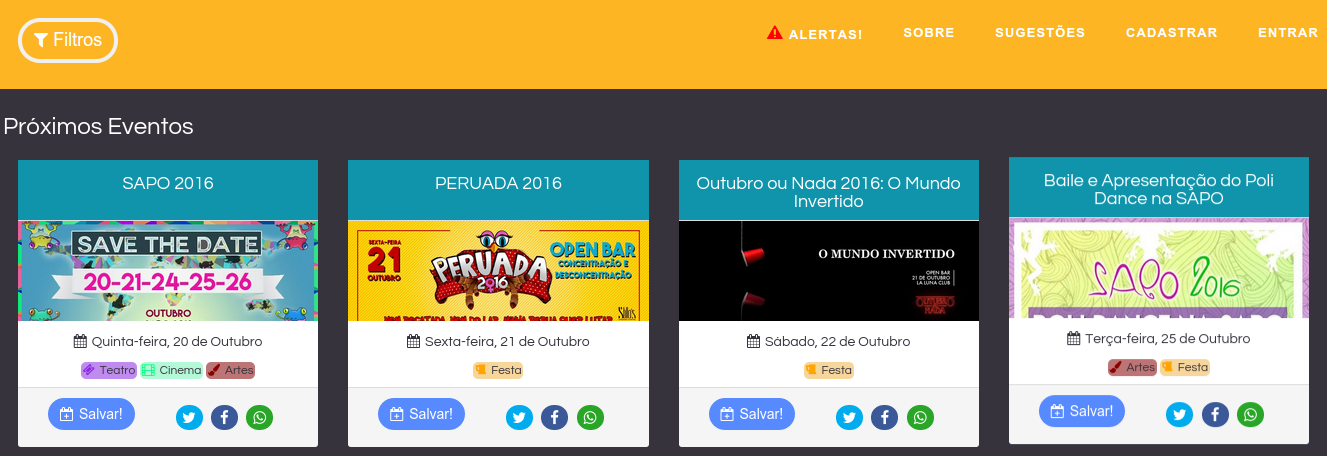
\includegraphics[width=15cm]{figuras/events_page_3aiteracao}
\caption{\label{fig:events_page_3aiteracao} Página de Eventos após modificações}
\end{figure}
	\par Victor Krug também afirma em seu livro que os usuários costumam criar ``mapas mentais'' de navegação sendo importante manter as convenções com o intuito de aproveitar-e dessa similaridade.
	\par Tomando como um exemplo de convenção o Sympla \footnote{Site: www.sympla.com.br} desde o começo nosso fluxo de navegação estava bastante próximo a convenção establecida: Uma página principal de Eventos contendo toda uma listagem de eventos sendo que cada evento direciona para sua própria página específica.
	\par Para aproximar ainda mais o fluxo de navegação foi incluída também na página inicial uma listagem com os ``Próximos Eventos'' assim como o Sympla faz com seus ``Eventos em Destaque''.
	\par Além disso foram implementados alguns efeitos visuais para chamar atenção do usuário:
	\begin{itemize}
	\item Ao passar o mouse sobre evento uma animação de salto do \emph{thumbnail} era rapidamente exibida.
	\item Ao carregar ou atualizar uma listagem de eventos seu carregamento era feito por meio de uma animação iniciada lateralmente.
	\end{itemize}
	\par A maior dificuldade em realizar o \emph{upload} de imagens foi o seu local de armazenamento pois o heroku não permite salvar arquivos em seu servidor, apenas armazenar em \emph{cache} durante a sessão, então foi feita a opção de criar uma conta de dropbox habilitada para receber imagens de aplicativos e integrá-la com a aplicação USP Eventos.

\subsection{Métricas}

\par Nessa iteração foi adicionado um Mapa de Calor (figura \ref{fig:heatmap}) para medir os cliques de mouse na página principal de eventos.
\begin{figure}[htb]
\centering
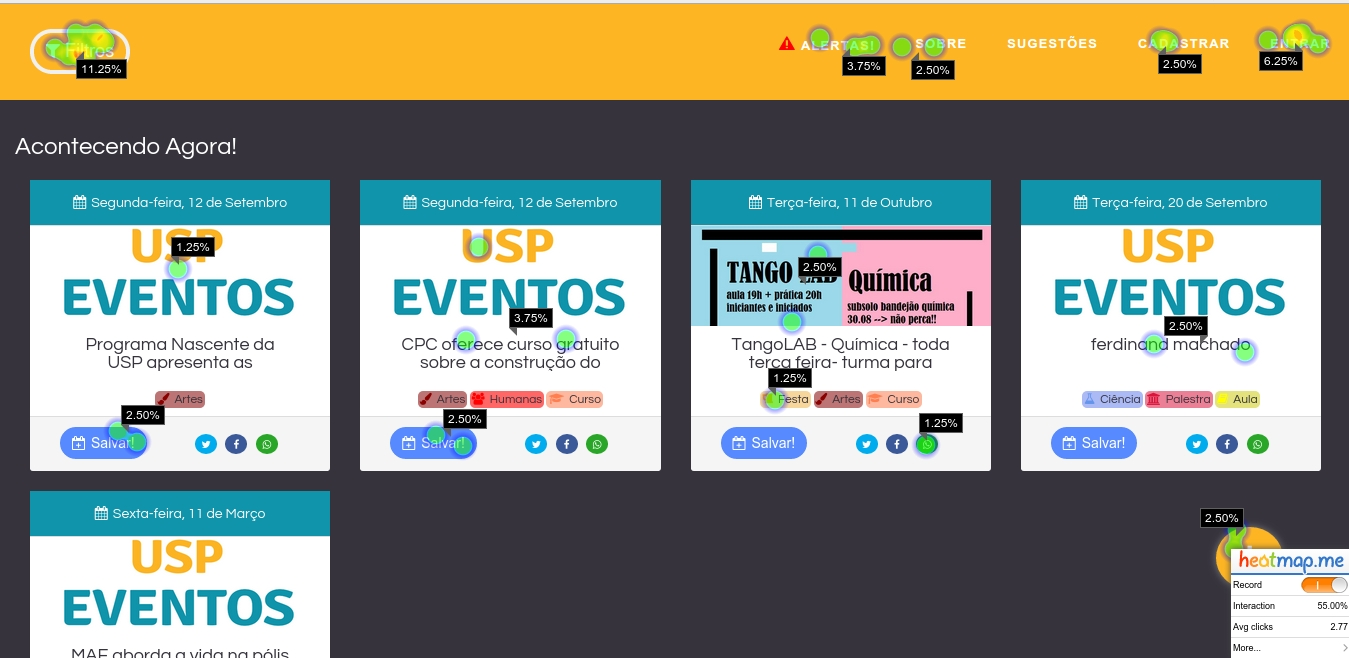
\includegraphics[width=15cm]{figuras/heatmap}
\caption{\label{fig:heatmap} Página principal de Eventos com o Mapa de Calor ativado}.
\end{figure}

\par Foi interessante observar que o Filtro estava sendo bastante utilizado tanto que em dado momento atingiu 40\% dos cliques na página.
\begin{figure}[htb]
\centering

\includegraphics[width=10cm]{figuras/heatmap_filter}
\caption{\label{fig:heatmap_filter} Botão de Filtro com 40\% dos cliques da página}.
\end{figure}

\par Outro ponto interessante observado é que muitos usuários também clicavam nas imagens dos eventos para acessar suas páginas de informações individuais mostrando que adicionar uma imagem para captar atenção do usuário trouxe resultados.

\par O enunciado de cada listagem foi clicado repetidas vezes pelos usuário o que pode significar que ele esteja sendo confundido com um \emph{link} (figura \ref{fig:heatmap_missclick}).
\begin{figure}[htb]
\centering

\includegraphics[width=10cm]{figuras/heatmap_missclick}
\caption{\label{fig:heatmap_missclick} Nome da Listagem: possível confusão com um link}.
\end{figure}
\par O Mapa de Calor foi incluído no site utilizando o serviço fornecido pelo site Heatmap.

\par Analisando os dados (figura \ref{fig:analytics_3ainteracao_dados}) obtidos pelo Analytics no período de 27/09 até 28/10 é possível observar uma diminuição na taxa de rejeição no site para 21,64\% e um aumento considerável no número de páginas visitadas e duração média por sessão.
\begin{figure}[htb]
\centering
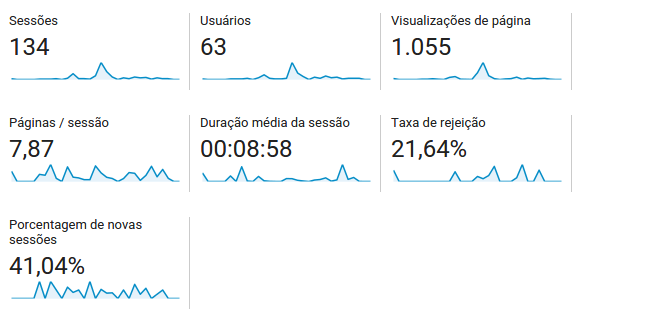
\includegraphics[width=15cm]{figuras/analytics_3ainteracao_dados}
\caption{\label{fig:analytics_3ainteracao_dados} Dados obtidos pelo G.A no período de 27/09 até 28/10 }.
\end{figure}

\par Ainda sim não houve grande crescimento no número de acesso e sessões totais.

\par Nesse período também ocorreram 92 cliques no botão de Salvar um Evento além de 424 cliques para utilizar a página de alertas.
\subsection{Aprendizado}
\par Com o intuito de realizar uma coleta de dados mais direta com os candidatos foi criado um Formulário utilizando o TypeForm e conversas com pessoas que utilizavam a plataforma.
\par Ao responder a pergunta ``Qual ou quais foram os maiores pontos positivos na sua opinião?'' a interface do site foi elogiada diversas vezes mostrando que as modificações foram de fato bem aceitas, algumas das respostas:
\par ``Interface bem fácil e intuitiva''\\
\par ``Organizar visualmente a informação dos eventos e a utilização de labels.''\\
\par ``intuitivo em sua maioria, bonito, fácil de entender como funciona''\\
\par ``Mostrar eventos de diversos temas (não só festas, por exemplo). Mas também, a
opção de selecionar os assuntos de sua preferência, ao fazer o cadastro.A interface é simples e clara, acho que atende aos objetivos e permite uma visualização rápida, podendo rolar até o mês desejável rapidamente.''\\
\par ``Reunir todos os eventos do campus em um só lugar.''\\
\par ``Gostei da preocupação em se fazer um site responsivo, já que, por ter inclusive uma seção Acontecendo Agora, é de se esperar que o acesso por meios móveis seja maior.''\\

\par Também foi feita uma pergunta sobre os pontos negativos e foi observado que alguns usuários acreditavam que os filtros não estivessem funcionando.
\par Conversando pessoalmente foi identificado uma confusão na forma como o filtro é aplicado.
\par Como o filtro é aplicado somente nas listagens de ``Eventos Acontecendo Agora'' e ``Próximos Eventos'' esses usuários não percebiam a filtragem estava sendo realizada.
\par Ainda sobre os filtros aparentemente não ficou claro para os usuários que ao preencher suas preferências durante o cadastro isso iria criar uma listagem personalizada com o nome de ``Principais Escolhas''.
\par Alguns comentários sobre os filtros:
\par ``No meu computador o site demora a responder e alguns filtros não funcionaram.''\\
\par ``Tentei usar o filtro e não funcionou mto bem.''\\

\par A página de Alertas também pareceu deslocada. Muitos não entenderam sua função e comentaram que o seu \emph{layout} atual está ruim.
\par Segue uma compilação das sugestões de funcionalidades recebidas:
\begin{itemize}
\item Filtros por data (dias da semana, próximos dias, etc).
\item Integrar com o Google Agenda
\item Integrar com os Eventos do Facebook (poder importar eventos do facebook para a plataforma)
\item Presença de um calendário
\item Campo de busca por extenso
\item Mapa com a localização dos Eventos
\item Sistema para disparar alertas ou lembretes para determinado evento.
\item Opção de cadastros oficiais, como uma certificação de que aquele perfil pertece a um Centro Acadêmico oficialmente por exemplo.
\item Feed de Notícias
\item Sistema de Avaliação para Eventos mais esperados
\item Vídeos e fotos pós evento
\end{itemize}

\par Algumas respostas sobre sugestões para a plataforma:
\par ``talvez criar mais uma separação ``eventos nos próximos 7 dias'' ou ``eventos dessa semana'', visualização de mapa?''\\
\par ``Senti falta de uma visualização dos eventos em um calendário.''\\
\par ``podia linkar com os eventos do fb! e já salvar nos seus eventos do fb.''\\
\par ``Talvez, um campo de busca para que fosse possível escolher um mês ou fim de semana específico...É rápido ir rolando a tela, mas para eventos a longo prazo, a barra de busca cumpriria melhor a função.''\\

\par Ao todo 25 pessoas responderam ao questionário, sendo que todas acreditam que uma plataforma centralizando Eventos na USP é de fato útil e  apenas 3 não gostaram do USP Eventos.
\par Dentre as críticas das 3 pessoas que não gostaram os seguintes pontos foram levantados:
\begin{itemize}
\item Acreditam que poucas pessoas hoje em dia usariam um site e talvez uma iniciativa dentro do Facebook fosse mais útil.
\item Ficaram incomodadas com a paleta de cores.
\item Gostariam de poder visualizar os eventos na página inicial.
\end{itemize}

\par A abordagem utilizando um questionário e conversas diretas trouxe uma quantidade muito maior de informação sobre a plataforma do que nas iterações anteriores mostrando que o Desenvolvimento do Cliente é realmente útil para direcionar o desenvolvimento do Sistema.
\par Utilizar um Mapa de Calor foi um acréscimo importante na coleta de dados pois foi possível perceber detalhes na forma como o usuário utiliza a plataforma tornando-se mais uma opção para realizar a validação da hipótese inicial.
\par A divulgação ainda parece ser não estar atingindo um grande número de pessoas resultando em um baixo volume de acessos.
